\chapter{Merge Sort}

\section{Introduzione}
Introduciamo il secondo algoritmo studiato durante il corso. Merge Sort è un algoritmo completamente diverso da Insertion Sort, in quanto è ricorsivo e non ordina sul posto (cioé ha bisogno di una quantità di memoria direttamente proporzionale alla lunghezza $n$ dell'array da ordinare). 

Il suo funzionamento (così come quello di tutti gli algoritmi ricorsivi) è basato sul divide et impera, cioé scomporre un macroproblema in tanti sottoproblemi di più facile risoluzione, fino ad arrivare ad un caso base banalmente risolubile, per poi tornare indietro sfruttando il caso base raggiunto.

Merge Sort funziona in due fasi diverse: la prima fase consiste nel dividere a metà l'array da ordinare, mentre nella seconda fase è presente la fusione ordinata delle due metà di array.

Bisogna dividere ricorsivamente l'array fin quando non arriviamo al caso base (array di un solo elemento), per poi risalire la catena fondendo in maniera ordinata questi mini-array ottenuti, fino ad ottenere di nuovo l'array originale ma ordinato; per fare ciò, quindi, abbiamo bisogno di copie di questi mini-array (quindi la memoria richiesta è proporzionale alla lunghezza dell'array stesso).

\section{Tempo di esecuzione}
%A differenza di Insertion Sort, Merge Sort ha bisogno di due procedure diverse per funzionare; le presentiamo di seguito.
%
%\begin{algorithm}
%\begin{algorithmic}[1]
%	\Procedure{MergeSort}{$A, p, r$}
%	\If{$p < r$}
%	\State $q \gets \lfloor (p+r) / 2 \rfloor $
%	\State MergeSort$(A,p,q)$
%	\State MergeSort$(A,q+1,r)$
%	\State Merge$(A,p,q,r)$
%	\EndIf
%	\EndProcedure
%\end{algorithmic}
%\end{algorithm}
%
%\begin{algorithm}
%\begin{algorithmic}[1]
%	\Procedure{Merge}{$a, p, q, r$}
%	\State $n1 \gets q-p+1$\Comment{Dimensione array sinistra}
%	\State $n2 \gets r-q$\Comment{Dimensione array destra}
%	
%	\For{$i \gets 1$ to $n1$}
%	\State $L[i] \gets A[p+i-1]$\Comment{Copia il sottovettore di sinistra in L}
%	\EndFor
%	
%	\For{$j \gets 1$ to $n2$}
%	\State $R[j] \gets A[q+j]$\Comment{Copia il sottovettore di destra in R}
%	\EndFor
%	
%	\State $L[n1+1] \gets R[n2+1] \gets +\infty$\Comment{Elemento sentinella}
%	
%	\State $i \gets j \gets 1$
%	
%	\For{$k \gets p$ to $r$}\Comment{Copia l'elemento più piccolo in A[k]}
%	\If{$L[i] \leq R[j]$}
%	\State $A[k] \gets L[i]$
%	\State $i \gets i+1$
%	\Else
%	\State $A[k] \gets R[j]$
%	\State $j \gets j+1$ 
%	\EndIf
%	\EndFor
%	
%	\EndProcedure
%\end{algorithmic}
%\end{algorithm}
%
%Come prima, analizziamo rapidamente lo pseudocodice per capire qual è il tempo di esecuzione atteso.
%
%La procedura MergeSort divide logicamente l'array in due fin quando i sotto-array non sono di dimensione unitaria. Supponendo l'array di partenza di dimensione $n$, otteniamo 2 array di dimensione $n/2$ dopo una chiamata di MergeSort, poi 4 array di dimensione $n/4$ dopo due chiamate, e così via fino ad avere n array di dimensione 1 dopo $log_{2}(n)$ chiamate di MergeSort. 
%
%Dopo aver diviso gli array con MergeSort, chiamiamo la funzione Merge, che consiste nel prendere due sotto-array adiacenti per fonderli in ordine nell'array. 
Il Merge Sort ha un tempo di esecuzione $T(n) = \Theta(n\log n)$. È peggiore del caso migliore dell'Insertion Sort, ma è un algoritmo migliore, - per quanto riguarda il tempo di esecuzione, ma non lo spazio occupato - in quanto il suo limite asintotico superiore è inferiore a quello di Insertion Sort, che è quadratico.

Come possiamo vedere nella figura \ref{merge:fig}, il tempo di esecuzione (a parte essere molto piccolo anche per dimensioni molto elevate dell'array da ordinare) cresce seguendo rigorosamente la traiettoria di $f(n) = an\log n$, con $a = 1.5*10^{-5}$.

\begin{figure}[h]
	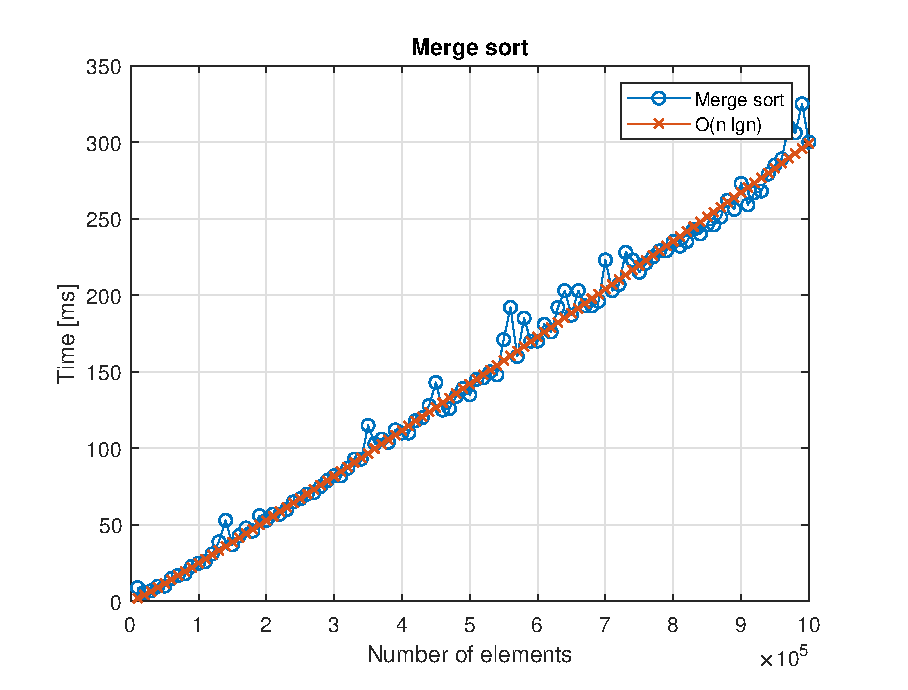
\includegraphics{merge/graph.eps}
	\captionAlgorithm{Merge Sort}
	\label{merge:fig}
\end{figure}
